% Evidence-Gated Edge Decoder -- architecture figure for FraudGT extension.
% Style mimics FraudGT Fig. 2 (dashed, colour-coded component outlines).
%
% Standalone build:   pdflatex evidence_gate_arch.tex
% In the ACM paper:    drop the \begin{figure*}...\end{figure*} block below into
%                      the document (it needs the same \usepackage lines).
%
\documentclass[border=6pt]{standalone}
\usepackage{amsmath}
\usepackage{tikz}
\usetikzlibrary{arrows.meta,positioning,fit,backgrounds,calc}

% --- palette (matches the SVG) ---
\definecolor{cBase}{HTML}{1F77B4}
\definecolor{cProto}{HTML}{2CA02C}
\definecolor{cStruct}{HTML}{D2691E}
\definecolor{cGate}{HTML}{7E57C2}
\definecolor{cFuse}{HTML}{D62728}
\definecolor{cEnc}{HTML}{555555}

\begin{document}
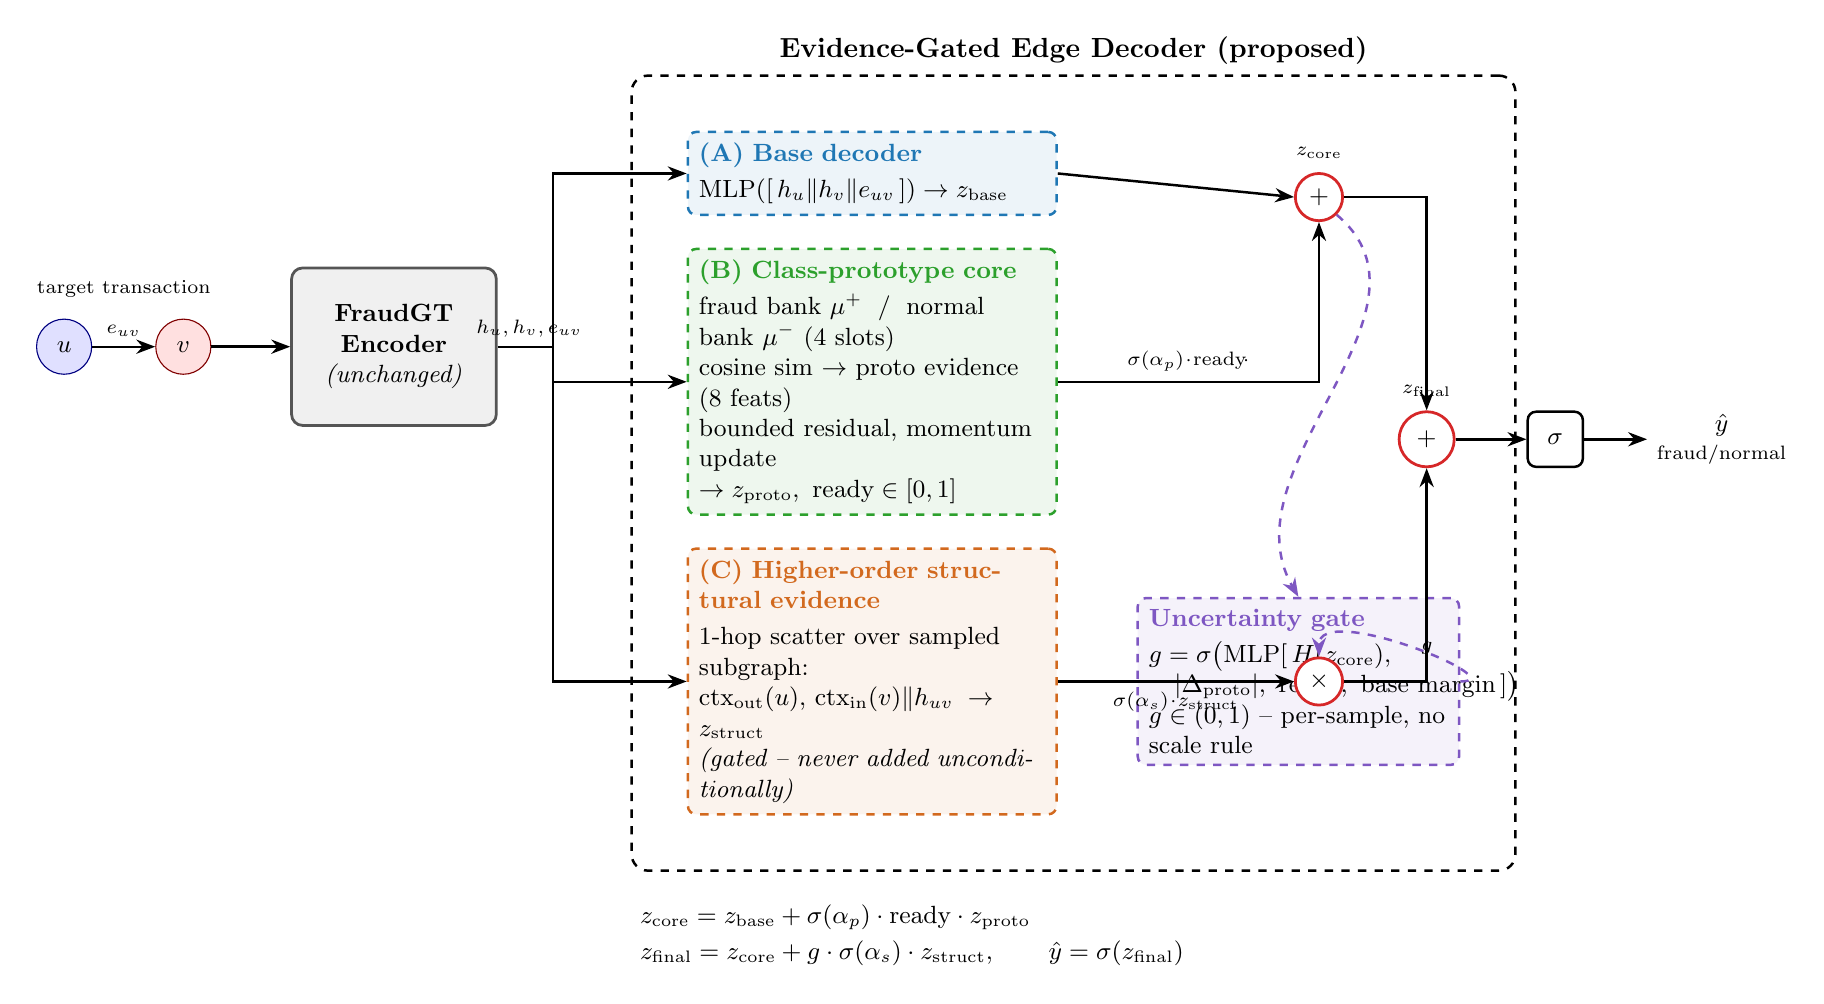
\begin{tikzpicture}[
  font=\small,
  >={Stealth[length=2.4mm]},
  comp/.style={rounded corners=3pt, draw, dashed, line width=0.9pt, align=left,
               inner sep=4pt},
  enc/.style={rounded corners=4pt, draw=cEnc, line width=1pt, fill=black!6,
              align=center, minimum width=26mm, minimum height=20mm},
  op/.style={circle, draw=cFuse, line width=1pt, fill=white, inner sep=0pt,
             minimum size=6mm},
  flow/.style={->, line width=0.9pt},
  gflow/.style={->, line width=0.9pt, draw=cGate, dashed},
]

% ---------------- input transaction ----------------
\node (u) [circle, draw=blue!50!black, fill=blue!12, minimum size=7mm] at (0,0) {$u$};
\node (v) [circle, draw=red!50!black,  fill=red!12,  minimum size=7mm, right=8mm of u] {$v$};
\draw[->, line width=0.8pt] (u) -- node[above,font=\scriptsize]{$e_{uv}$} (v);
\node[font=\scriptsize, above=5mm of $(u)!0.5!(v)$] {target transaction};

% ---------------- encoder ----------------
\node (enc) [enc, right=10mm of v] {\textbf{FraudGT}\\\textbf{Encoder}\\\textit{(unchanged)}};
\draw[flow] ($(v.east)$) -- (enc.west);

% ---------------- decoder components ----------------
\node (base) [comp, draw=cBase, fill=cBase!8, right=24mm of enc, yshift=22mm,
              text width=44mm] {%
  {\color{cBase}\textbf{(A) Base decoder}}\\[2pt]
  $\mathrm{MLP}([\,h_u\Vert h_v\Vert e_{uv}\,]) \to z_{\text{base}}$};

\node (proto) [comp, draw=cProto, fill=cProto!8, below=4mm of base, text width=44mm] {%
  {\color{cProto}\textbf{(B) Class-prototype core}}\\[2pt]
  fraud bank $\mu^{+}$ \;/\; normal bank $\mu^{-}$ (4 slots)\\
  cosine sim $\to$ proto evidence (8 feats)\\
  bounded residual, momentum update\\
  $\to z_{\text{proto}},\ \text{ready}\in[0,1]$};

\node (struct) [comp, draw=cStruct, fill=cStruct!8, below=4mm of proto, text width=44mm] {%
  {\color{cStruct}\textbf{(C) Higher-order structural evidence}}\\[2pt]
  1-hop scatter over sampled subgraph:\\
  $\mathrm{ctx}_{\text{out}}(u),\,\mathrm{ctx}_{\text{in}}(v)\Vert h_{uv} \to z_{\text{struct}}$\\
  \textit{(gated -- never added unconditionally)}};

\node (gate) [comp, draw=cGate, fill=cGate!8, right=10mm of struct, text width=38mm] {%
  {\color{cGate}\textbf{Uncertainty gate}}\\[2pt]
  $g=\sigma\big(\mathrm{MLP}[\,H(z_{\text{core}}),$\\
  $\quad |\Delta_{\text{proto}}|,\ \text{ready},\ \text{base margin}\,]\big)$\\
  $g\in(0,1)$ -- per-sample, no scale rule};

% dashed container around the proposed decoder
\begin{scope}[on background layer]
  \node (box) [draw, dashed, rounded corners=6pt, line width=0.9pt,
    fit=(base)(proto)(struct)(gate), inner sep=7mm] {};
\end{scope}
\node[anchor=south, font=\bfseries] at (box.north) {Evidence-Gated Edge Decoder (proposed)};

% feed edge representation from encoder into the three components
\coordinate (bus) at ($(enc.east)+(7mm,0)$);
\draw[line width=0.8pt] (enc.east) -- (bus);
\node[font=\scriptsize, above] at ($(enc.east)+(4mm,0)$) {$h_u,h_v,e_{uv}$};
\draw[flow] (bus) |- (base.west);
\draw[flow] (bus) |- (proto.west);
\draw[flow] (bus) |- (struct.west);

% ---------------- fusion ----------------
\node (sum1) [op, right=30mm of base.east, yshift=-3mm] {$+$};
\node[font=\scriptsize, above=0.5mm of sum1] {$z_{\text{core}}$};
\node (mul)  [op] at (sum1 |- struct) {$\times$};
\node (sum2) [op, minimum size=7mm, right=10mm of $(sum1)!0.5!(mul)$] {$+$};
\node[font=\scriptsize, above=0.5mm of sum2] {$z_{\text{final}}$};
\node (sig)  [rounded corners=3pt, draw, line width=0.9pt, right=9mm of sum2,
             minimum size=7mm] {$\sigma$};
\node (yhat) [right=8mm of sig, align=center] {$\hat{y}$\\[-1pt]{\scriptsize fraud/normal}};

\draw[flow] (base.east)  -- (sum1.west);
\draw[flow] (proto.east) -| node[pos=0.25,above,font=\scriptsize]{$\sigma(\alpha_p)\!\cdot\!\text{ready}\!\cdot$} (sum1.south);
\draw[flow] (struct.east) -- node[below,font=\scriptsize]{$\sigma(\alpha_s)\!\cdot\! z_{\text{struct}}$} (mul.west);
\draw[gflow] (gate.east) to[out=0,in=90] node[right,font=\scriptsize]{$g$} (mul.north);
\draw[gflow] (sum1.south east) to[out=-40,in=120] (gate.north);
\draw[flow] (sum1.east) -| (sum2.north);
\draw[flow] (mul.east)  -| (sum2.south);
\draw[flow] (sum2.east) -- (sig.west);
\draw[flow] (sig.east)  -- (yhat.west);

% ---------------- equation legend ----------------
\node[anchor=north west, align=left, font=\small] at ($(box.south west)+(0,-3mm)$) {%
  $z_{\text{core}} = z_{\text{base}} + \sigma(\alpha_p)\cdot\text{ready}\cdot z_{\text{proto}}$\\[2pt]
  $z_{\text{final}} = z_{\text{core}} + g\cdot\sigma(\alpha_s)\cdot z_{\text{struct}},
   \qquad \hat{y}=\sigma(z_{\text{final}})$};

\end{tikzpicture}
\end{document}
